\section{Reactor Models}
\label{sec:reactor_models}

This thesis explores various transition scenarios for the deployment in the \gls{usa} of the: 1) \gls{xe} \gls{htgr}; 2) \gls{usnc} \gls{mmr} \gls{htgr}; and 3) and Westinghouse AP1000 \gls{pwr}. To accommodate the assumption that the \gls{haleu}-fueled \gls{triso} reactors will first accept \gls{leup} fuel, this thesis adapts Bachmann's \gls{mmr}-like Serpent model \cite{bachmann_mmr_like_2023} and Richter's \gls{xe}-like Serpent model \cite{richter_xe100_like} to accept \gls{leup} fuel. These reactor models are constructed from publicly available data to approximate their aggregate behavior.

Table \ref{tab:ar_defs} shows the design specifications for the advanced reactors in this thesis. The \gls{mmr} and \gls{xe} reactors are \gls{htgr}s that use \gls{triso} fuel, while the AP1000 is a \gls{pwr} that uses UO$_2$ fuel. The enrichment distinguishes the versions of the \gls{mmr} and \gls{xe} as the only distinguishing variable between the two versions of the reactors. The cycle length, discharge burnup, and reactor lifetime are the same for both versions of the reactors. The AP1000 is assumed to use \gls{leu} fuel throughout the simulation. The \gls{mmr} is the smallest power output reactor in this thesis, and can serve as a representative of mix of small, \gls{triso}-fueled reactors. The \gls{xe} reactor is an order of magnitude larger in power output, and can be considered a representative of larger, \gls{triso}-fueled reactors. The AP1000 is the largest reactor in this thesis and is a representative of gigawatt-scale reactors.


\begin{table}[H]
   \centering
   \caption{Advanced reactor design specifications.}
   \label{tab:ar_defs}
   \begin{tabular}{l l l l}
      \hline
      \textbf{Design Criterion} & \textbf{MMR-Like} \cite{usnc_design_2021} & \textbf{\gls{xe}-Like} \cite{nuscale_chapter_2018} & \textbf{AP1000} \\
      \hline
      Reactor type & \gls{htgr} & \gls{htgr} & \gls{pwr} \\
      Power Output [MWe] & 15 & 100 & 1000 \\
      Fuel Type & \gls{triso} & \gls{triso} & UO$_2$ \\
      Enrichment [\% $^{235}$U] & 9.95, 19.75 & 9.95, 15.5 & 5 \\
      Cycle Length & 20 [yrs] & Online Refuel & 18 [months] \\
      Discharge Burnup [GWd/MTU] & 82 & 168 & 65 \\
      Reactor Lifetime [yrs] & 20 & 60 & 60 \\
      \hline
   \end{tabular}
\end{table}

The following subsections discuss the reactors in greater detail. These models  approximate that the \gls{leup}-fueled reactors achieve the same burnup, power level, and core lifetime as the \gls{haleu}-fueled version. These assumptions are sufficient for the metrics outlined in Section \ref{sec:metrics} as this thesis does not perform \gls{uf} isotopic analysis, but could stretch the \gls{uf} temporal profile.



\subsection{MMR-like Reactor}
\label{sec:mmr}

In 2021, \gls{uiuc} submitted a notice of intent to the \gls{nrc} detailing their plans to apply for a construction permit of the \gls{mmr} reactor from \gls{usnc} \cite{uiuc_notice_nrc_2021}. Activities have continued as \gls{uiuc} continues the project, they reached the pre-licensing phase with the \gls{nrc} and were planning on commencing operation of an on-campus reactor in the 2030s. This \gls{mmr} is an \gls{htgr} that uses \gls{triso} fuel, has an electrical output of 15 MW$_e$, and a cycle length of 20 years. The fuel is enriched to 9.95\% $^{235}$U for \gls{leup} and 19.75\% for \gls{haleu}. As modeled, both have a discharge burnup of 82 GWd/MTU, which coincides with the 20-year lifetime of the reactor. In this thesis, the \gls{mmr} is based on the model developed by Bachmann et al. \cite{bachmann_mmr_like_2023} and is implemented here as-is for the \gls{haleu} version of the reactor, while the \gls{leup} version updates the fuel composition from the \gls{haleu} version.

Figure \ref{fig:mmr_design} shows a rendering of the \gls{mmr} core and reactor vessel. As indicated by the figure, the design is intended to be underground, with an estimated total reactor footprint less than 5 acres. The primary coolant is helium gas, which heats up in the core and deposits its heat in a heat exchanger to generate electricity to the side of the reactor \cite{usnc_chalk_river}. Helium is transparent to many nuclear interactions and is inert, making it an attractive choice for a coolant.

\begin{figure}[H]
    \centering
    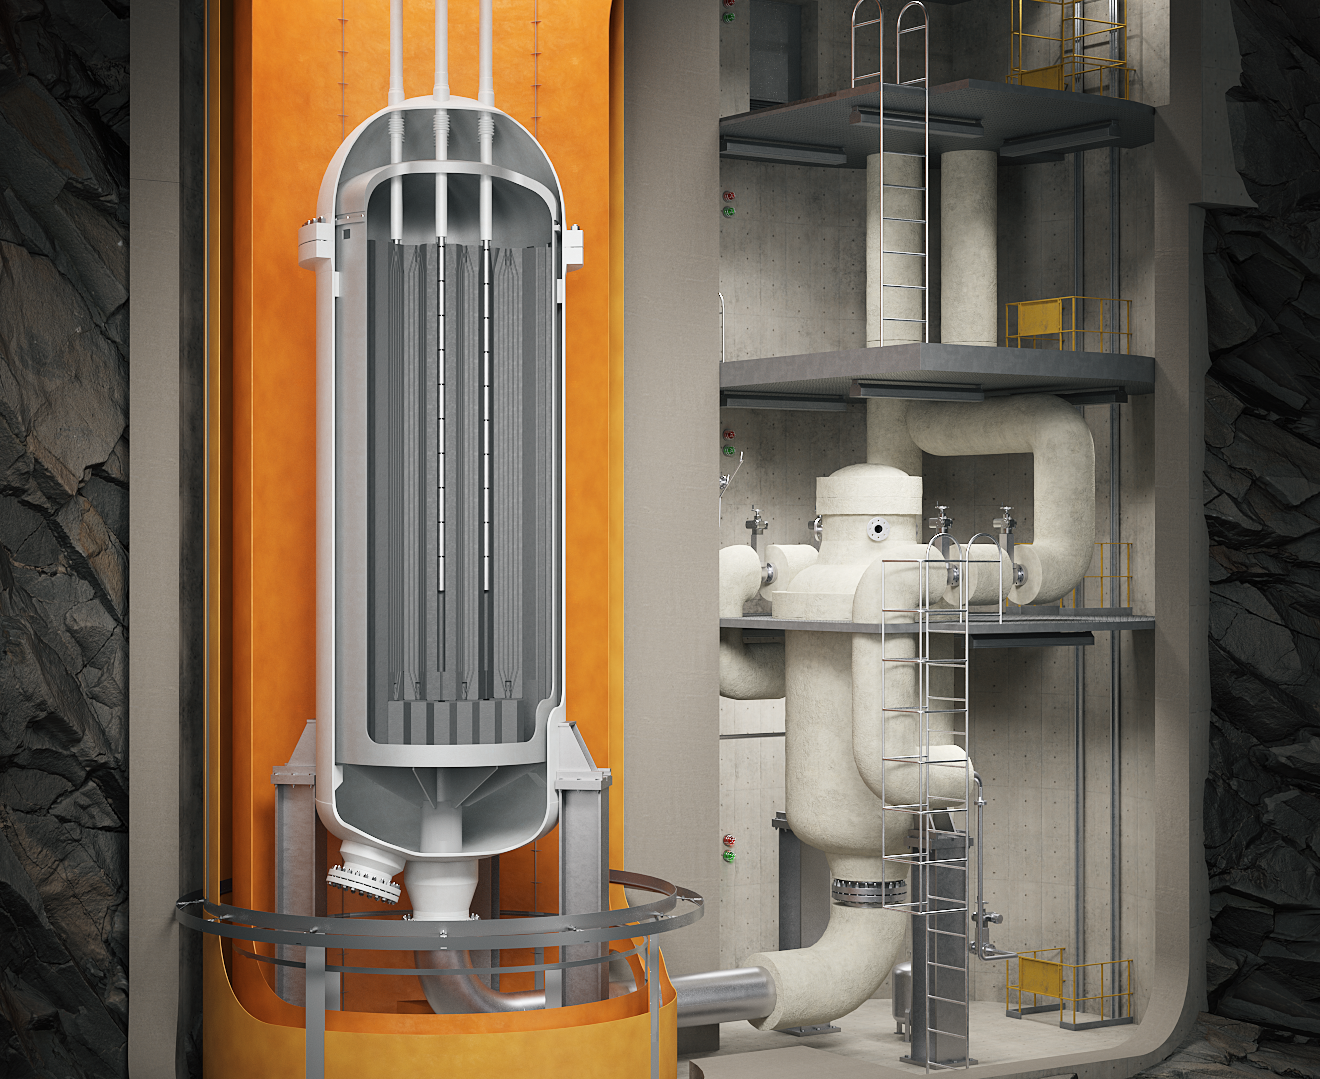
\includegraphics[scale=0.19]{images/reactor_design/wide-02.png}
    \caption{USNC MMR design \cite{usnc_design_2021}.}
    \label{fig:mmr_design}
\end{figure}

The proposed deployment of this reactor concept includes an operational \textit{\gls{mmr} Energy System} consisting of two plants: the \textit{Nuclear Plant} and the \textit{Adjacent Plant}. The \textit{Nuclear Plant} contains multiple \gls{mmr} units, including all the equipment required to transport the heat to the \textit{Adjacent Plant}. The \textit{Adjacent Plant} consists of the equipment that converts heat to electricity or process heat as needed. The \textit{\gls{mmr} Energy System} will theoretically store up to 10 hours of power plant thermal output and can be supplemented with hydrogen burners. Auxiliary molten salt thermal storage allows for a flexible electricity and process heat supply.

Electricity and heat would be delivered on demand from the power plant while the \gls{mmr} unit operates at constant power. The \gls{mmr}'s high-temperature heat has many uses beyond the generation of electricity. District heating, desalination, and chemical or industrial heat highlight the broader point of how \gls{geniv} nuclear reactors are not solely intended for electricity generation as with the current domestic fleet. An \gls{mmr} could deliver steam temperatures of 660 °C, and they estimate that temperatures up to 950 °C could be possible in future \gls{mmr} variants \cite{usnc_design_2021}.

The fuel for this reactor is inspired by the \gls{triso} fuel developed in the 1960s and 1970s. A small sphere of uranium fuel is coated in carbon and silicon carbide layers. As shown in Figure \ref{fig:usnc_fuel}, the fuel is composed of kernels arranged into a larger fuel pellet. They call their fuel form \gls{fcm} fuel. They additively manufacture each element, allowing for a high packing fraction of fuel, which means their fuel could be adapted to other reactor designs.

\begin{figure}[H]
    \subfloat[Fuel element layers.\label{fig:elemenet_layers}]{%
      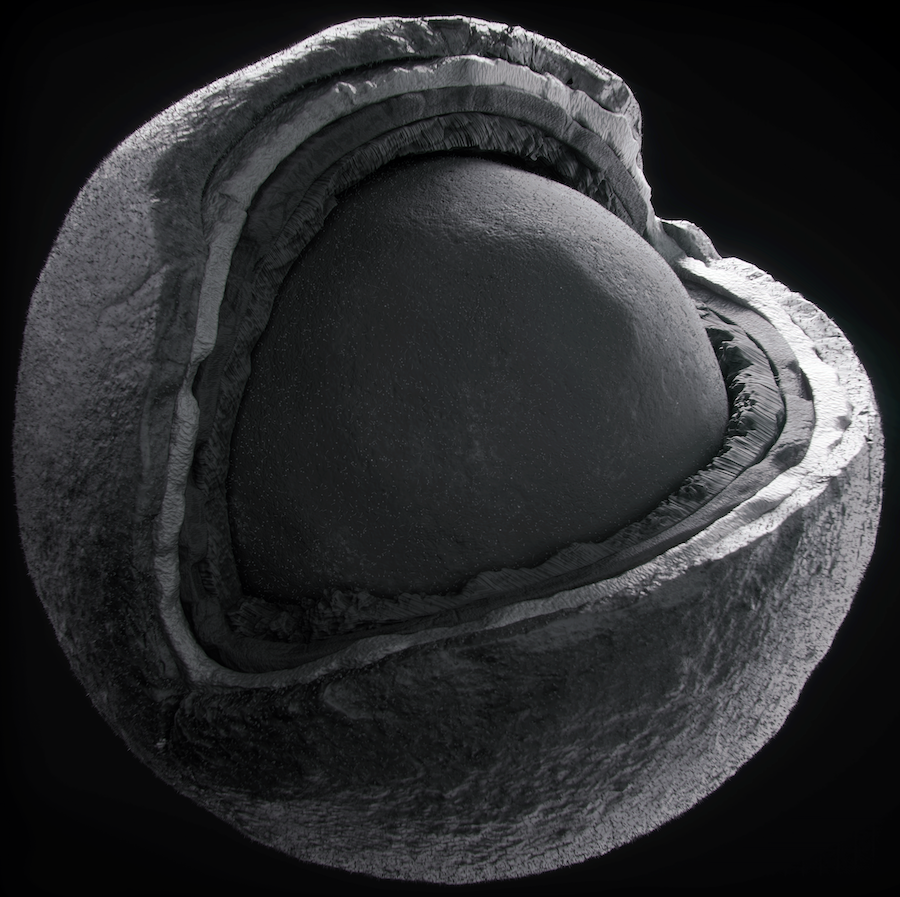
\includegraphics[width=0.49\textwidth]{images/reactor_design/usnc_triso.png}
   }
    \hfill
    \subfloat[Fuel pellet profile.\label{fig:pellet_profile}]{%
      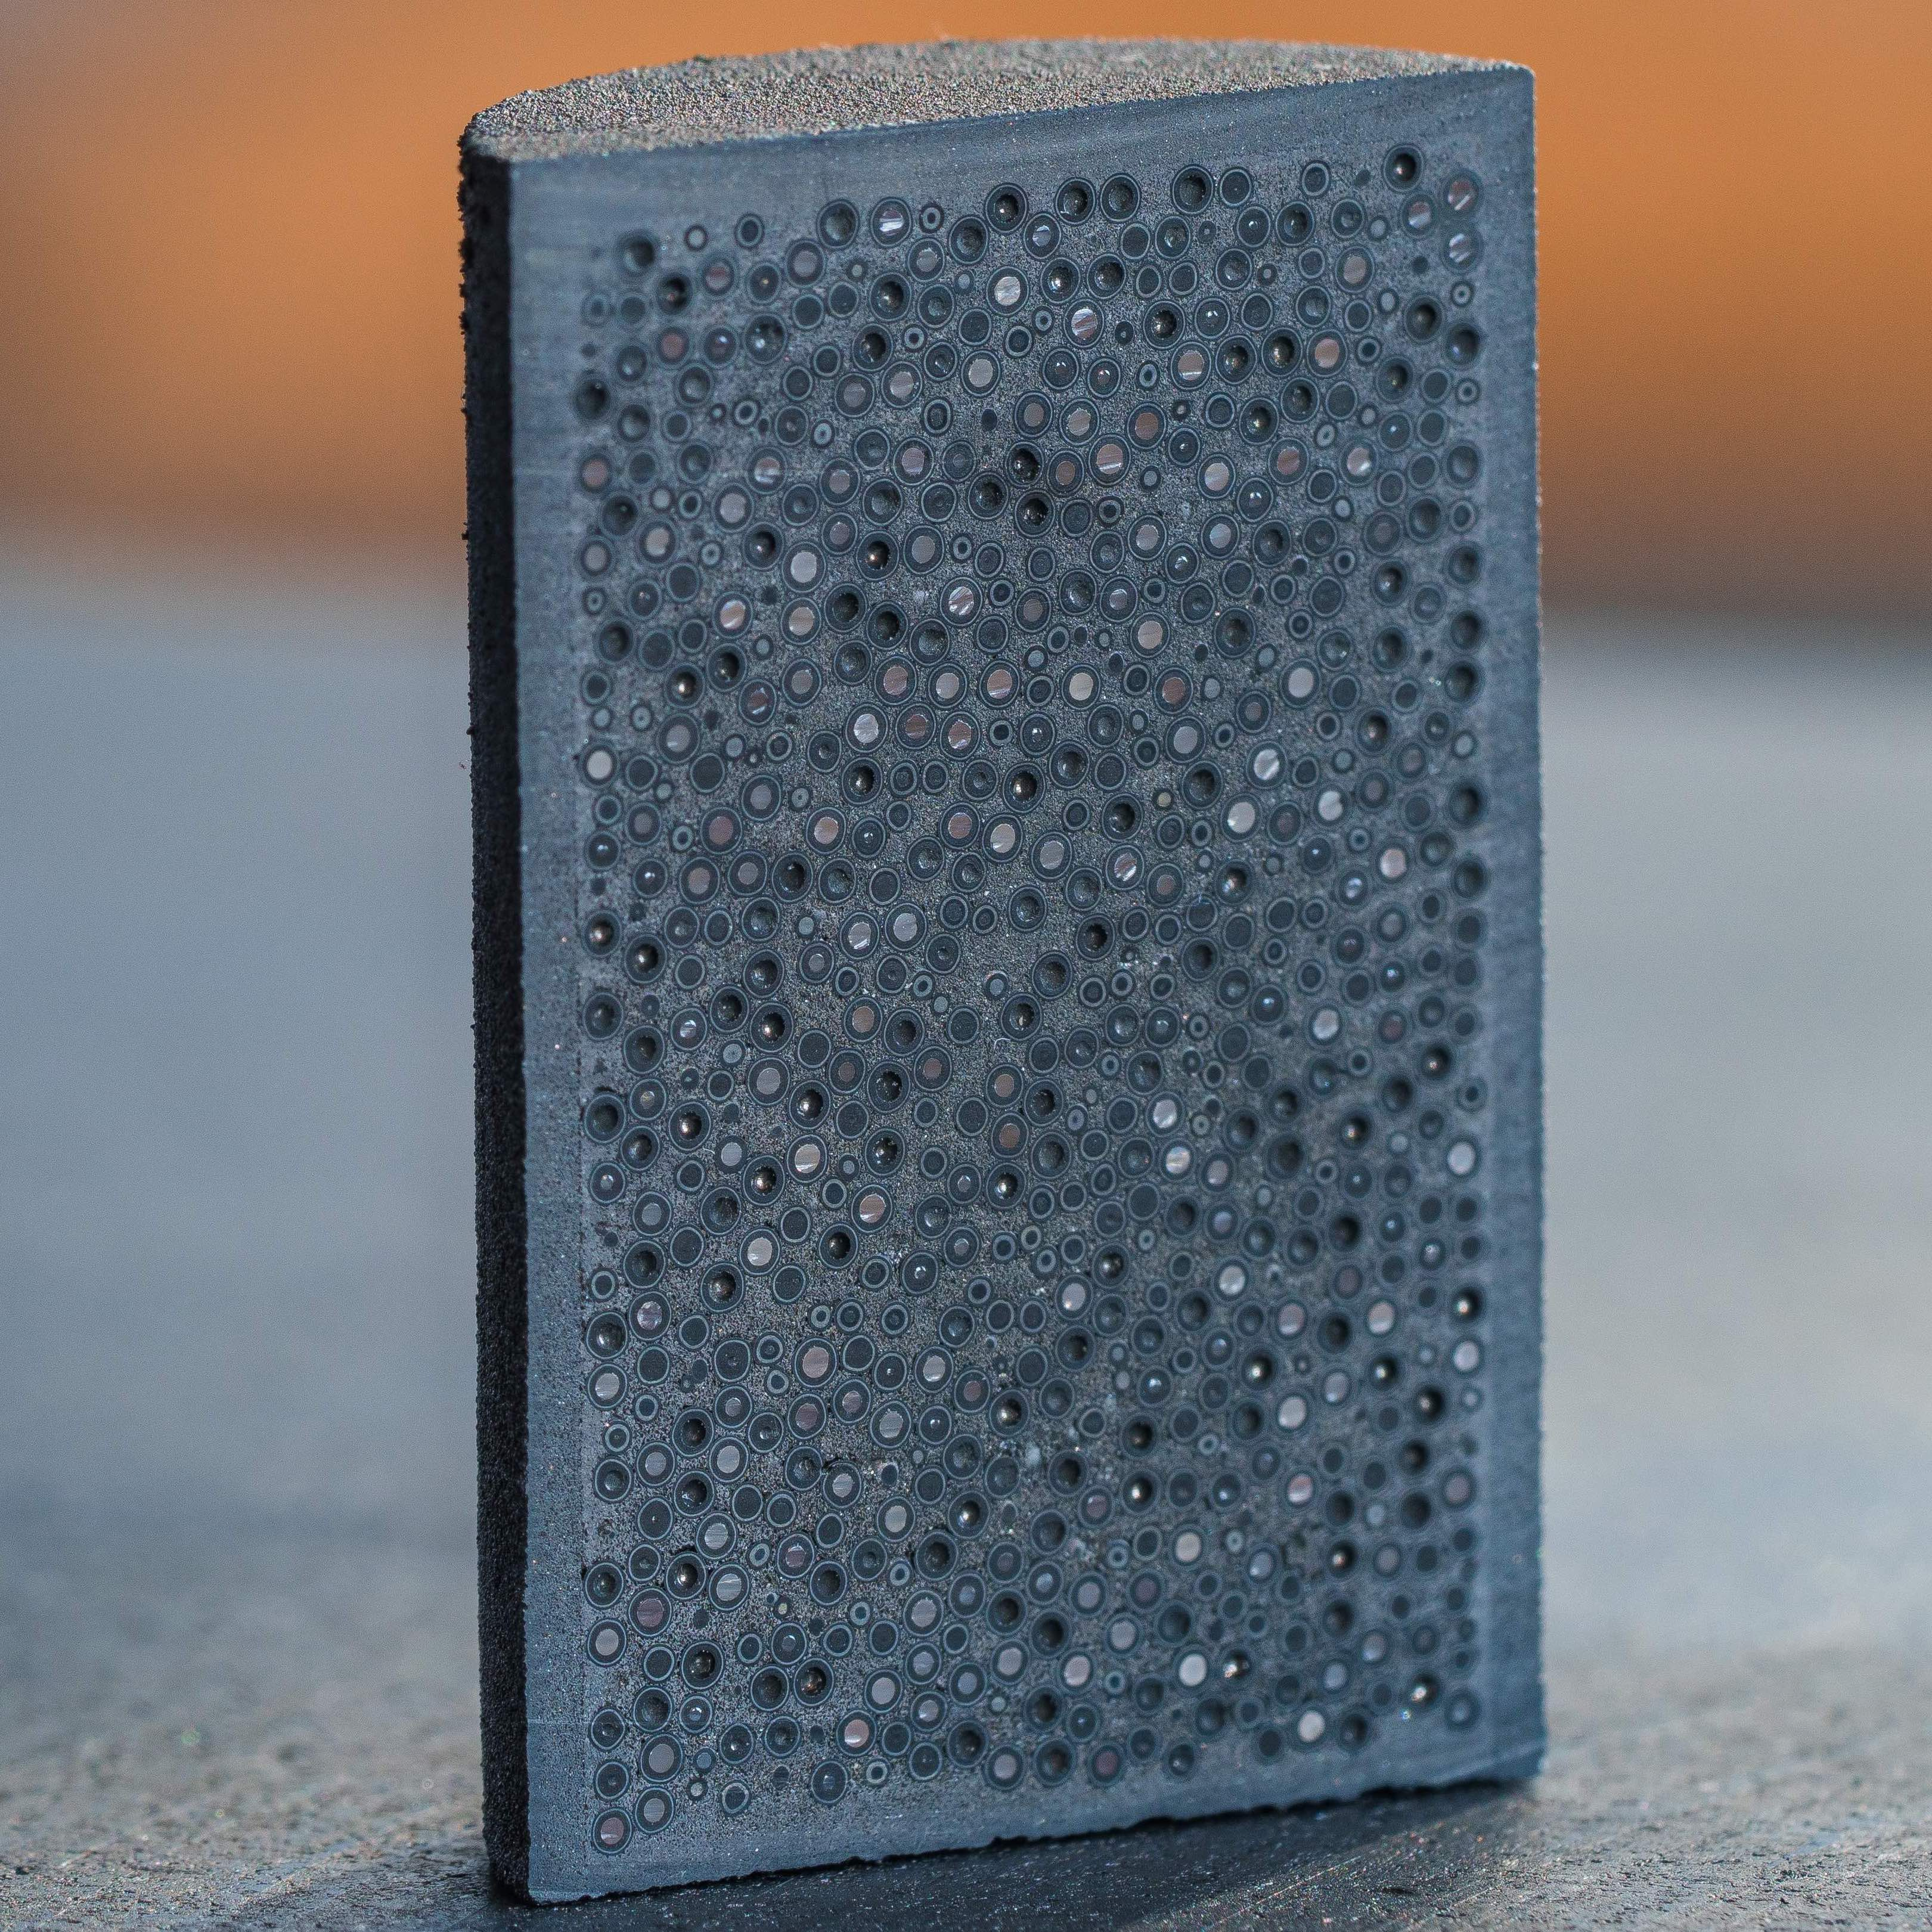
\includegraphics[width=0.49\textwidth]{images/reactor_design/usnc_fuel_side.jpeg}
   }
    \caption{
    USNC \gls{mmr} fuel renderings
      \cite{usnc_media_kit}.}
    \label{fig:usnc_fuel}
\end{figure}

Figure \ref{fig:mmr_core} shows a top-down and side view of the \gls{mmr} Serpent model \cite{bachmann_mmr_like_2023}, modified in fuel composition alone. As Bachmann describes \cite{bachmann_thesis_2023}, the radius of the fuel channel is based on the publicly available size of the \gls{fcm} pellets (1.15 cm), and the coolant channel has an arbitrarily chosen radius of 3 cm. The entire core is assumed to be in an isothermal state at 800 K. There is a 20 cm thick graphite reflector above and below the stacks of graphite and a 10 cm thick beryllium-oxide reflector on the outside of the graphite blocks of the core, illustrated by the green material in Figure \ref{fig:mmr_core}. The model does not contain control rods or burnable poisons, so the control rod tubes are filled with helium. Five layers of graphite fuel blocks are stacked to form the entire core to approximate the number of fuel blocks described in the publicly available data \cite{usnc_design_2021}. The fuel does not move through the core, as the model is designed to use the same fuel for the entire reactor lifetime.


\begin{figure}[H]
    \subfloat[Top-down core view.\label{fig:mmr_td}]{%
      
\includegraphics[width=0.49\textwidth]{images/reactor_design/haleu_mmr_2blocks.inp_geom1.png}
   }
    \hfill
    \subfloat[Full core side profile.\label{fig:mmr_slice}]{%
      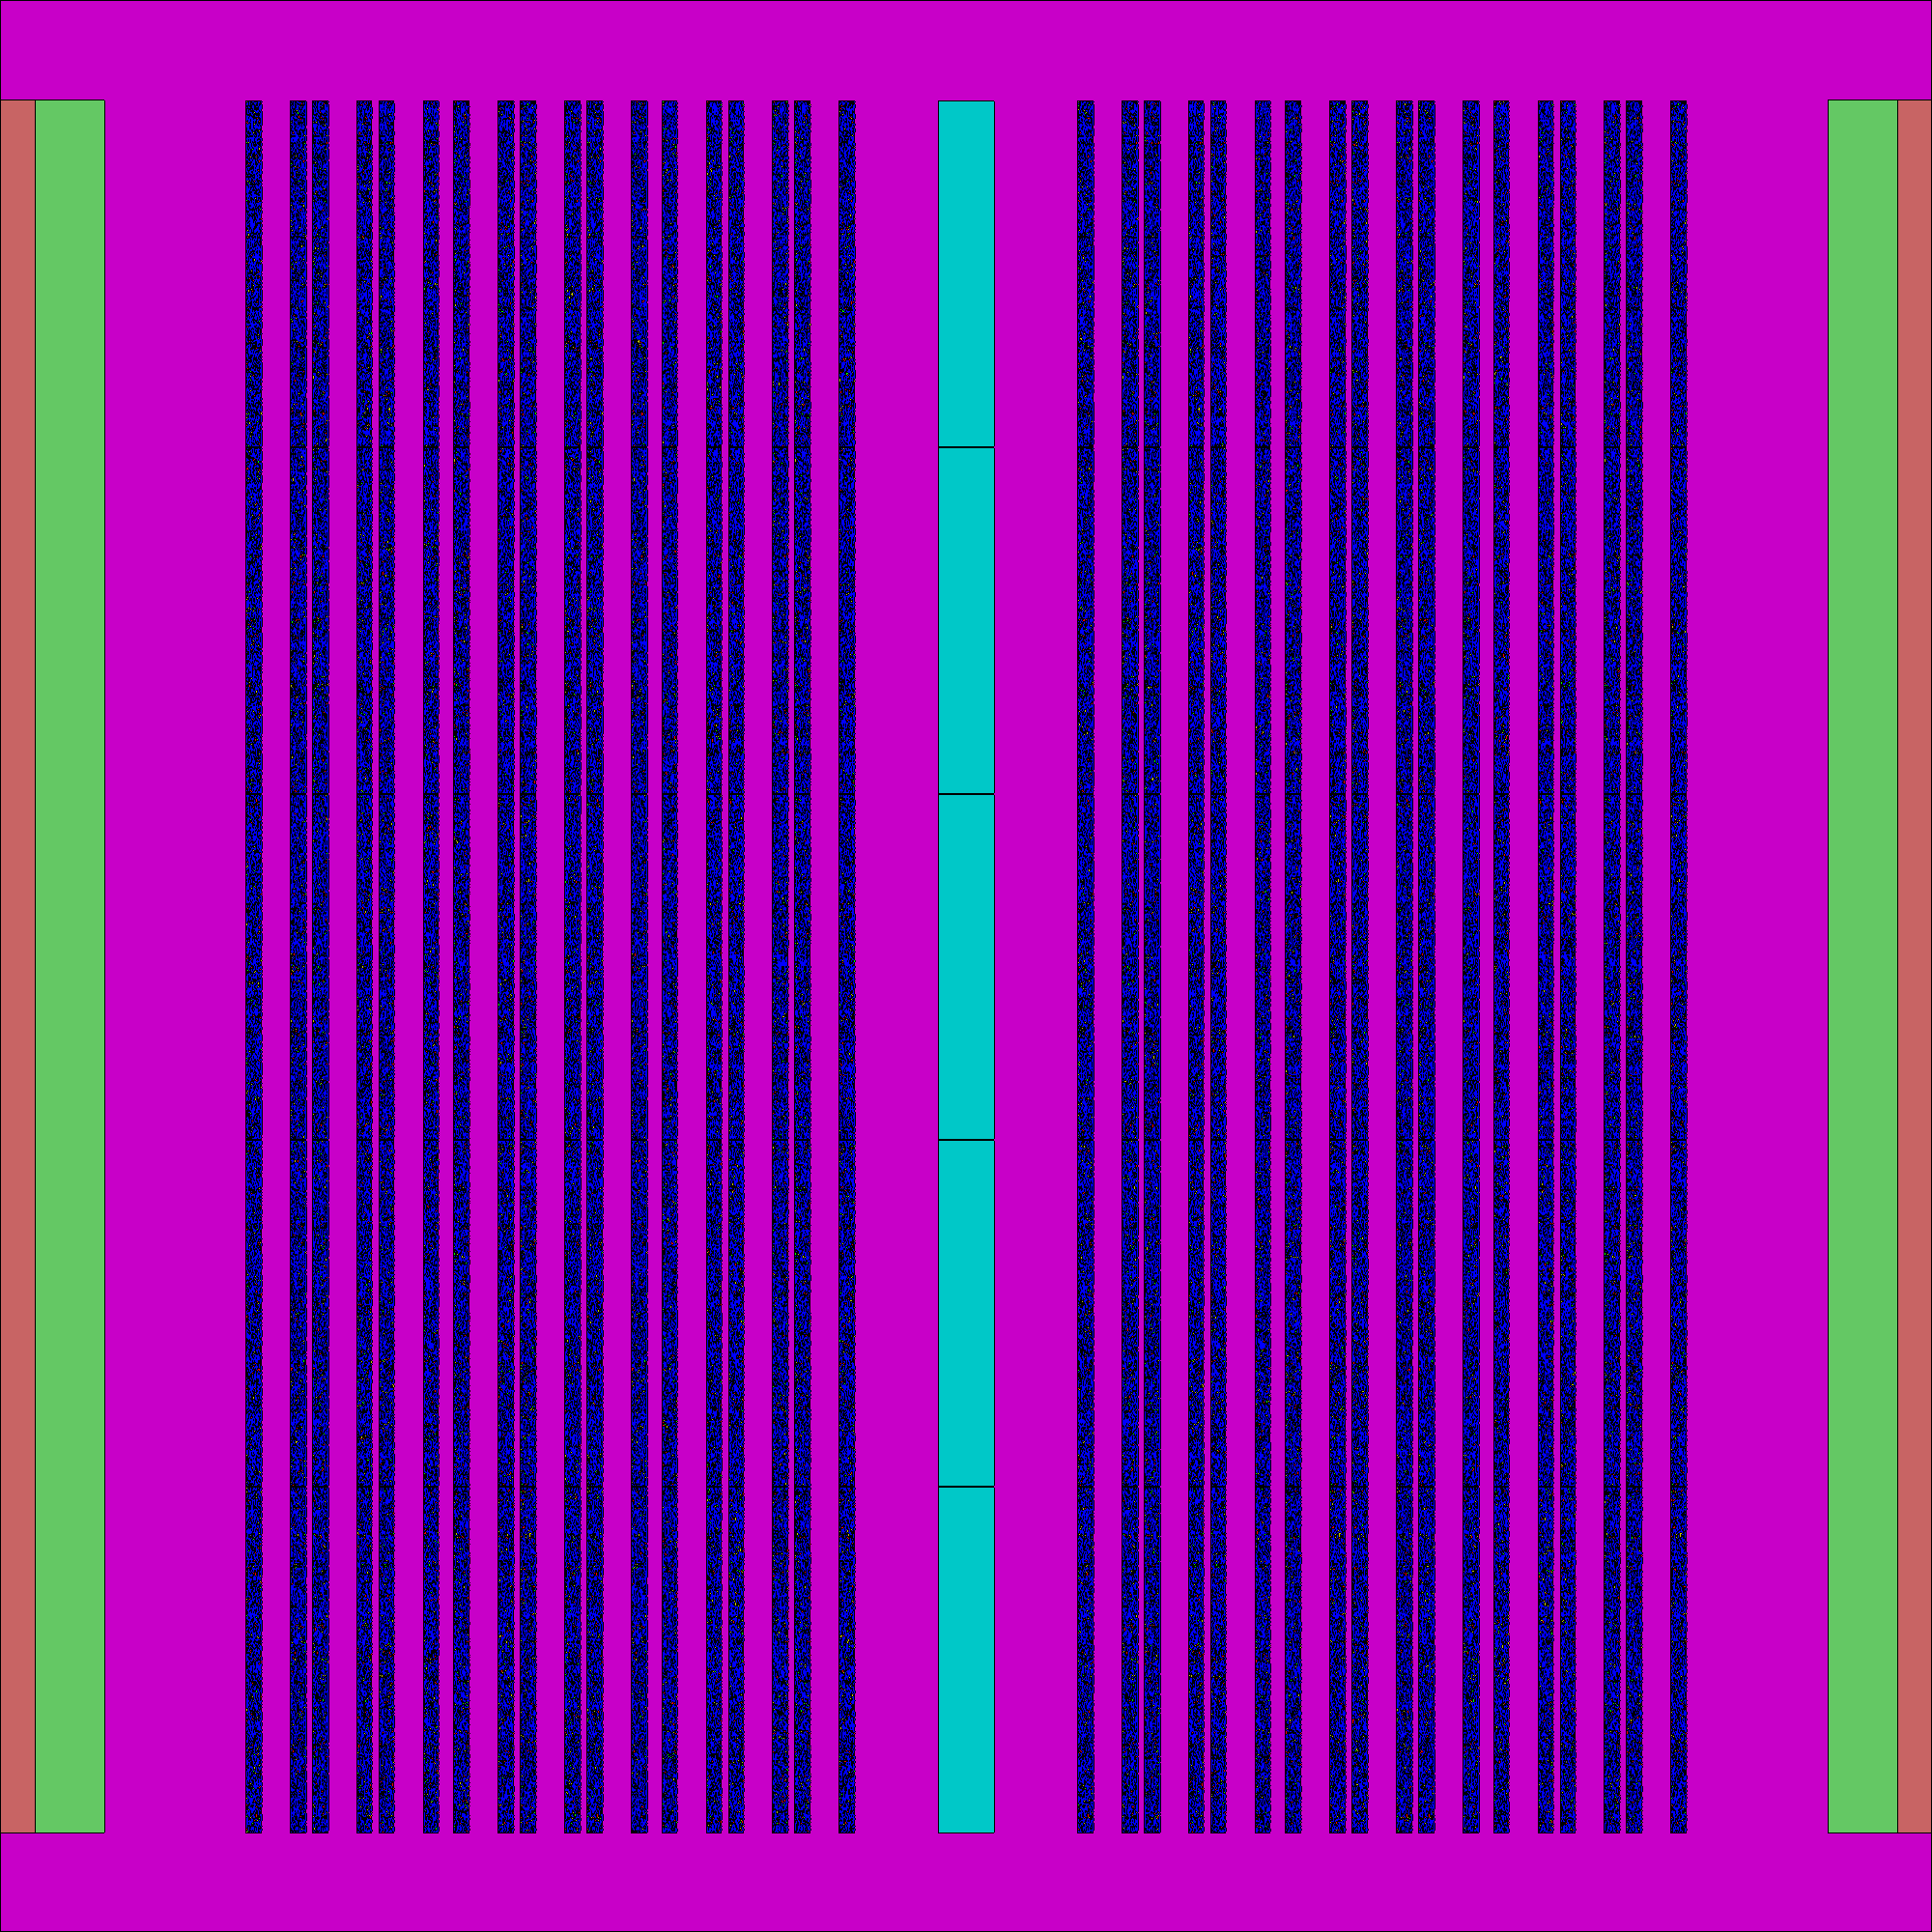
\includegraphics[width=0.49\textwidth]{images/reactor_design/haleu_mmr_2blocks.inp_geom3.png}
   }
    \caption{Serpent model of the USNC MMR core.}
    \label{fig:mmr_core}
\end{figure}



\subsection{Xe-100-like Reactor}
\label{sec:xe}

X-Energy has entered into a cooperative agreement with \gls{doe} to deploy their \gls{xe}, is in the pre-licensing phase with the \gls{nrc} for projects in Texas and Washington, and is expected to be operational in the 2030s. There are similar projects in the early stages in Canada and the \gls{uk}. The X-Energy \gls{xe} is an \gls{htgr} that uses \gls{triso} fuel and is expected to operate for 60 years. The reactor has an electical output of 100 MW and uses online refueling. The fuel is enriched to 9.95\% $^{235}$U for \gls{leup} and 15.5\% $^{235}$U for \gls{haleu} and a discharge burnup of 168 GWd/MTU. The reactor in this thesis is an approximation based on publicly available data and is not based on confidential or proprietary information. The model was developed by Richter et al. \cite{richter_xe100_like} and is implemented herein as-is for the \gls{haleu}-fueled reactor, while the \gls{leup} version has a modified fuel composition.

Figure \ref{fig:xe_design} shows a rendering of the \gls{xe} core and reactor vessel. The \gls{xe} reactor is designed to be a small modular reactor that can be deployed in various locations and will be gas-cooled. This design differs from the \gls{mmr} as the reactor features online refueling.

\begin{figure}[H]
    \centering
    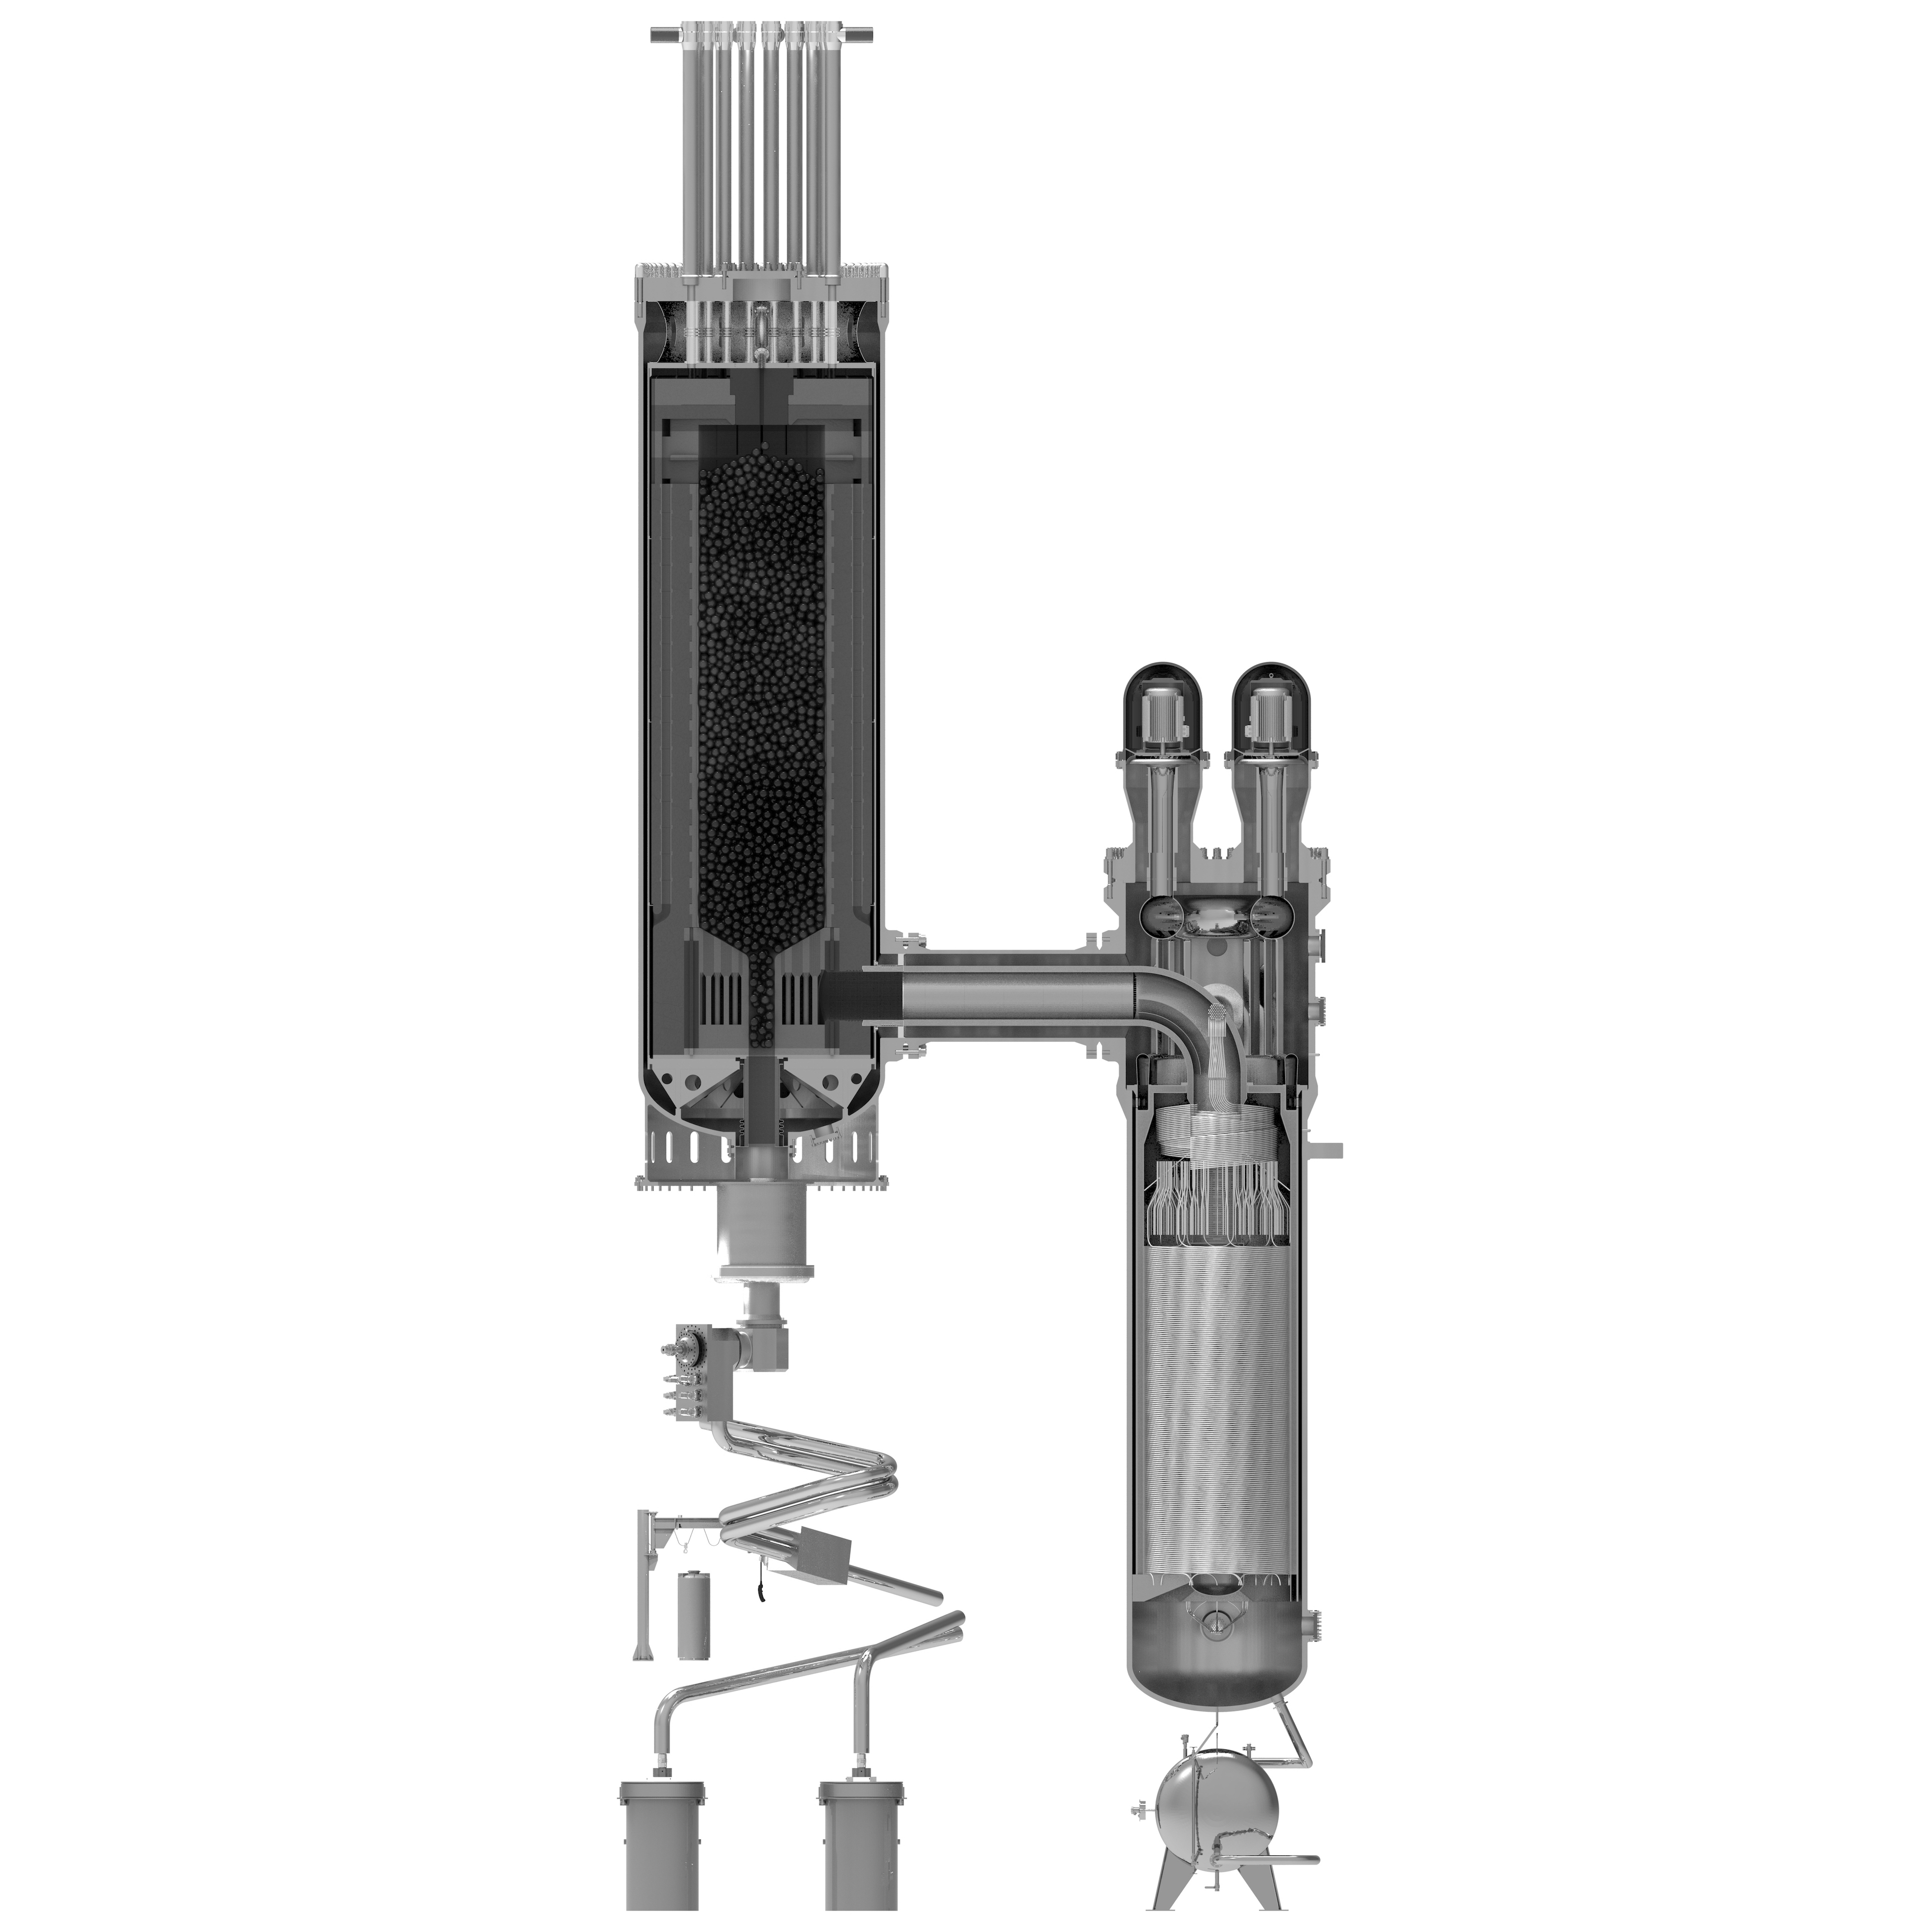
\includegraphics[scale=0.09]{images/reactor_design/xe-100-reactor-slice.jpg}
    \caption{X-Energy Xe-100 rendition \cite{xe_reactor}.}
    \label{fig:xe_design}
\end{figure}

Unlike the \gls{mmr}'s annular fuel elements, the \gls{xe} pebbles are composed of a spherical graphite matrix that contains the \gls{triso} fuel particles. These \gls{triso} particles are similar to those in the \gls{mmr}, as shown in Figure \ref{fig:xe_fuel}.

\begin{figure}[H]
    \centering
    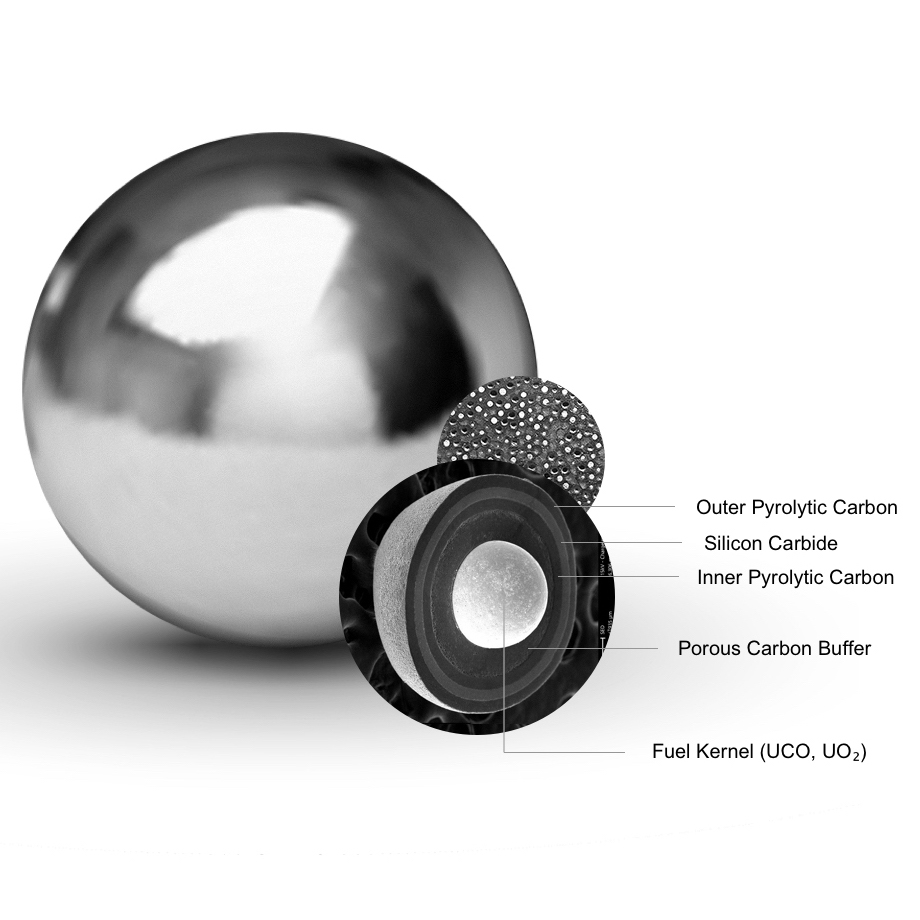
\includegraphics[scale=0.28]{images/reactor_design/graphic-triso-x-pebble.jpg}
    \caption{X-Energy Xe-100 fuel pebble \cite{xe_fuel}.}
    \label{fig:xe_fuel}
\end{figure}


This thesis modifies the fuel composition of Richter's \gls{xe}-like reactor model to accept \gls{leup} fuel. The \gls{leup} fuel is assumed to have the same burnup and power level as the \gls{haleu} fuel. This assumption, as with the \gls{mmr}-like reactor, would impact the \gls{uf} isotopic calculations. I will explore the implications in future work. Figure \ref{fig:xe_core} shows the top-down view of the \gls{leup} \gls{xe} core as the \gls{haleu} version has been established by Richter \cite{richter_thesis_2022}.

\begin{figure}[H]
    \subfloat[Initial core. \label{fig:xe_init_core}]{%
      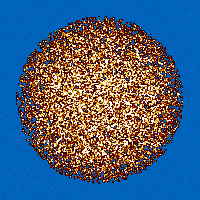
\includegraphics[width=0.49\textwidth]{images/reactor_design/htgr-mr-burn-200.inp_mesh1_bstep0.png}
   }
    \hfill
    \subfloat[Final core. \label{fig:xe_final_core}]{%
      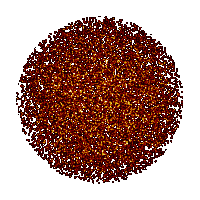
\includegraphics[width=0.49\textwidth]{images/reactor_design/htgr-mr-burn-200.inp_mesh1_bstep6.png}
   }
    \caption{Top-down view of the \gls{leup} X-Energy Xe-100 core model where darker shading corresponds to higher burnup, and lighter shading corresponds to lower burnup.}
    \label{fig:xe_core}
  \end{figure}

Figures \ref{fig:xe_init_core} and \ref{fig:xe_final_core} are shaded based on the burnup of the fuel, with darker pebbles indicating higher burnup. The pebbles are inserted into the core at the top, and gravity pulls them down through the core. After a brief holding time outside the core, the pebbles are reinserted at the top of the core. In \cyclus, we approximate the core as containing 6 batches in the core and one batch is removed when they reach the end of their life. This process is repeated until the pebbles reach their targeted number of passes, at which point they are removed from the core and stored.

\subsection{AP1000 Reactor}
\label{sec:ap}

AP1000s are operational in the \gls{usa} and China, and the \gls{uk} and India plan to deploy more. The Westinghouse AP1000 is a \gls{pwr} that uses UO$_2$ fuel. The reactor has an electrical output of 1000 MW, a cycle length such that every 18 months 80 fuel assemblies are replaced, and an expected lifetime of 60 years. The fuel is enriched to approximately 5\% $^{235}$U and has a discharge burnup of 65 GWd/MTU. The reactor in this thesis is an approximation based on publicly available data about the units currently operating at the Vogtle Plant in Georgia, and is not based on confidential or proprietary information. As this thesis does not anticipate \gls{leup} being used in the AP1000, there is no such neutronics model of the reactor herein, and this work adapts the generic \cycamore reactor archetype to represent the AP1000 in number of fuel assemblies, power output, core mass, and cycle length.
